\documentclass{sigchi}
% Use this command to override the default ACM copyright statement (e.g. for preprints). 
% Consult the conference website for the camera-ready copyright statement.

%% EXAMPLE BEGIN -- HOW TO OVERRIDE THE DEFAULT COPYRIGHT STRIP -- (July 22, 2013 - Paul Baumann)
% \toappear{Permission to make digital or hard copies of all or part of this work for personal or classroom use is 	granted without fee provided that copies are not made or distributed for profit or commercial advantage and that copies bear this notice and the full citation on the first page. Copyrights for components of this work owned by others than ACM must be honored. Abstracting with credit is permitted. To copy otherwise, or republish, to post on servers or to redistribute to lists, requires prior specific permission and/or a fee. Request permissions from permissions@acm.org. \\
% {\emph{CHI'14}}, April 26--May 1, 2014, Toronto, Canada. \\
% Copyright \copyright~2014 ACM ISBN/14/04...\$15.00. \\
% DOI string from ACM form confirmation}
%% EXAMPLE END -- HOW TO OVERRIDE THE DEFAULT COPYRIGHT STRIP -- (July 22, 2013 - Paul Baumann)


% Arabic page numbers for submission. 
% Remove this line to eliminate page numbers for the camera ready copy
\pagenumbering{arabic}


% Load basic packages
\usepackage{balance}  % to better equalize the last page
\usepackage{graphics} % for EPS, load graphicx instead
\usepackage{times}    % comment if you want LaTeX's default font
\usepackage{url}      % llt: nicely formatted URLs

% llt: Define a global style for URLs, rather that the default one
\makeatletter
\def\url@leostyle{%
  \@ifundefined{selectfont}{\def\UrlFont{\sf}}{\def\UrlFont{\small\bf\ttfamily}}}
\makeatother
\urlstyle{leo}


% To make various LaTeX processors do the right thing with page size.
\def\pprw{8.5in}
\def\pprh{11in}
\special{papersize=\pprw,\pprh}
\setlength{\paperwidth}{\pprw}
\setlength{\paperheight}{\pprh}
\setlength{\pdfpagewidth}{\pprw}
\setlength{\pdfpageheight}{\pprh}

% Make sure hyperref comes last of your loaded packages, 
% to give it a fighting chance of not being over-written, 
% since its job is to redefine many LaTeX commands.
\usepackage[pdftex]{hyperref}
\hypersetup{
pdftitle={SIGCHI Conference Proceedings Format},
pdfauthor={LaTeX},
pdfkeywords={SIGCHI, proceedings, archival format},
bookmarksnumbered,
pdfstartview={FitH},
colorlinks,
citecolor=black,
filecolor=black,
linkcolor=black,
urlcolor=black,
breaklinks=true,
}

% create a shortcut to typeset table headings
\newcommand\tabhead[1]{\small\textbf{#1}}


% End of preamble. Here it comes the document.
\begin{document}

\title{SIGCHI Conference Proceedings Format}

\numberofauthors{3}
\author{
  \alignauthor 1st Author Name\\
    \affaddr{Affiliation}\\
    \affaddr{Address}\\
    \email{e-mail address}\\
    \affaddr{Optional phone number}
  \alignauthor 2nd Author Name\\
    \affaddr{Affiliation}\\
    \affaddr{Address}\\
    \email{e-mail address}\\
    \affaddr{Optional phone number}    
  \alignauthor 3rd Author Name\\
    \affaddr{Affiliation}\\
    \affaddr{Address}\\
    \email{e-mail address}\\
    \affaddr{Optional phone number}
}

\maketitle

\begin{abstract}
In this paper we describe the formatting requirements for
SIGCHI Conference Proceedings, and this sample file
offers recommendations on writing for the worldwide
SIGCHI readership. Please review this document even if
you have submitted to SIGCHI conferences before, some
format details have changed relative to previous years.
\end{abstract}

\keywords{
	Guides; instructions; author's kit; conference publications;
	keywords should be separated by a semi-colon.
	\textcolor{red}{Mandatory section to be included in your final version.}
}

\category{H.5.m.}{Information Interfaces and Presentation (e.g. HCI)}{Miscellaneous}

See: \url{http://www.acm.org/about/class/1998/}
for more information and the full list of ACM classifiers
and descriptors. 
\textcolor{red}{Mandatory section to be included in your
final version. On the submission page only the classifiers'
letter-number combination will need to be entered.}

\section{Cooperative Game}

% Cooperative design has been an integral part of many games. With the success of games like Left4Dead,Portal 2,Gears of War, many game designers and producers are currently exploring the addition of cooperative patterns within their games.
% Cooperative Games encourage participation and collaboration, the goal is not to win as player but as a team of players. Discovering effective cooperative game patterns is an elusive and important problem.

In a growing diversity of generations, cooperative game has been an integral part of today's game development. There are a variety of great cooperative game such as Left4Dead, Portal 2, and Gears of War. With so many success cooperative game in the market, We can find out that it is a trend for game designers and related company to explore more and more cooperative patterns within their games. Cooperative games not only make players' collaboration but also result in players' higher game participation. To design a great cooperative game, the main idea is to win the game with team members rather than a single person. As we mentioned above, we know that it  is important for game designers to find out great cooperative patterns, but it also becomes a elusive problem to discover an effective cooperative game patterns.

% Some researchers analyzed a set of cooperative games to develop cooperative game design patterns. Zagal et al., for example, explored cooperative patterns within board games[1]. Also, Bjork and Holopainen presented a large number of game design patterns [2], which included cooperative and social interaction patterns.In addition Zagal et al, presented an ontology for analyzing game play [3]. Rocha et al. presented a framework of several cooperative game design patterns[4] .

In order to develop cooperative game design patterns, several researchers analyzed a set of cooperative games. For example, Zagal et al. explored cooperative patterns within board games \cite{1}, and it also presented an ontology with a view to analyzing game play \cite{3}; Bjork and Holopainen, which presented a large quantity of game design patterns \cite{2}, included cooperative and social interaction patterns; Rocha et al. presented a framework of several cooperative game design patterns \cite{4}.

% Special cases in cooperative game also become a exploring area. Wolmet et al.reports on a study of how parents and children play several cooperative co-located games with different characteristics[5]. Mark et al [6]. evaluate the communicative and cooperative behavior of same-age and mixed-age pairs (Young-Young, Young-Old, Old-Old),and identified noticeable differences between the group-types. Hamilton et al [7], explored how to design games for children with cerebral palsy to play ,and presents several cooperative gameplay prototypes.

We can realize some principle to generate cooperative game design patterns from many general cases. However, if we are eager to comprehend cooperative game design completely, some special cases in cooperative game are also an inevitable exploring area. For instance, Wolmet et al. reported a study of how parents and children play several cooperative co-located games with different characteristics \cite{5}; Mark et al. \cite{6} evaluated the communicative and cooperative behavior of same-age and mixed-age pairs (Young-Young, Young-Old, Old-Old), and identified noticable difference between group types; Hamilton et al. \cite{7} explored how to design games for children to play with cerebral palsy, and it also presented several cooperative gamplay prototypes.

% With rapid development of Internet, playing cooperative game with player from different country become a normal situation, but cooperative game for different language speaker is still an untapped area. In this work, we want to understand how language boundary affect cooperative game experience, and how to design a game that avoid negative game experience while playing with different language speaker.

With the rapid development of Internet, it is common for players to play cooperative games from different country. Nonetheless, players consist of different language speakers are still an untapped area for cooperative game design. In our work, we want to understand how language boundary affects cooperative game experience and how to design a game which can avoid negative gameplay experience while playing with different language speakers.



\section{Pilot Study}

% To understand how language boundary affect cooperative game experience, we recruit 9 Taiwaneses and 3 Japaneses and divided into 2 separate group-types(i)Taiwan-Taiwan, (ii)Taiwan-Japan. We have validated that Taiwanese players don’t understand Japanese and vise versa. We choose three different cooperative games on Steam[1] (so that player can talk to each other through Steam Talk), Rocketbirds:Hardboiled Chicken(Cooperative Action Game) ,Portal 2 (Cooperative Puzzle Game), Monaco (Cooperative Stealth Game).To emulate quick match via Internet, two players are playing these games at two distinct rooms using headphones for communication. Players play these three games 30 minutes for each. After playing each game, players will fill up an eSFQ[2] questionnaire for rapid assessment of game experiences and conduct an open-ended interviews.

In order to understand how language boundary affect cooperative game experience, we proceeded pilot study, added a factor of language boundary, for players to play the famous cooperative game on the market today. We recruited players with 9 Taiwaneses and 3 Japanese, and we divided them into 2 separated group-types: (i)Taiwan-Taiwan, (ii)Taiwan-Japan. We had confirmed that all Taiwanese players don't understand Japanese and vice versa. We choosed three different famous cooperative games: Rocketbirds:Hardboiled Chicken (Cooperative Action Game), Portal 2 (Cooperative Puzzle Game), Monaco (Cooperative Stealth Game). In addition, all three games were chosen from Steam\cite{PS1} so that players can talk to each other through Steam Talk. Besides, in order to emulate quick connection via Internet, both players were placed at two different rooms and used headphones to communicate with each other. Each time players proceed these three games for 30 minutes. Last but not least, we would like to assess game experiences and conducted an open-ended interviews, players had to fill up an eSFQ\cite{PS2} questionnaire after playing each game respectively.






\section{Game Design}

% Base on our pilot study results, we understand that if the cooperative game require High-Level Feature Communication, play it with non-common language player is really frustrating. According to GameFlow[1], games challenging should match the player’s skill level, If the challenges are greater than the skills, the result is anxiety and frustrating, if the challenges are less than the skills, the result is apathy and boring.

Based on our pilot study results(see Table 2), we realize that if playing cooperative games requires high-level-feature communication, playing with different language players would feel deeply frustrated. According to GameFlow\cite{GD1}, game challenges should match the player's skill level. If the challenges are greater than the player's skills, the gameplay result will be anxiety and frustrated. But, by constrast, if the challenges are less than the player's skills, the result will be apathy and bored.

% According to our observation, play cooperative game with different language speaker will significantly decrease cooperative skills which is really important for most cooperative games and the game challenge become too hard for this situation and causing frustrating. The most easy way to solve this problem is to decrease the game challenge difficulty for non-common language players, but it is not practical for commercial games because the players with common language would feel boring with no difficulty.

According to our observation, playing cooperative game with different language speaker will significantly decrease cooperative skills which is really important for most cooperative games. And game challenges would become too hard for this situation and cause frustrated. The easiest way to solve this problem is to decrease the game's difficulty for non-common language players. Nevertheless, this method is not practical for commercial games because it will make players with common language feel bored with no difficulty while playing the game (see Figure~\ref{fig:GD_F1}).  

\begin{figure}[!h]
\centering
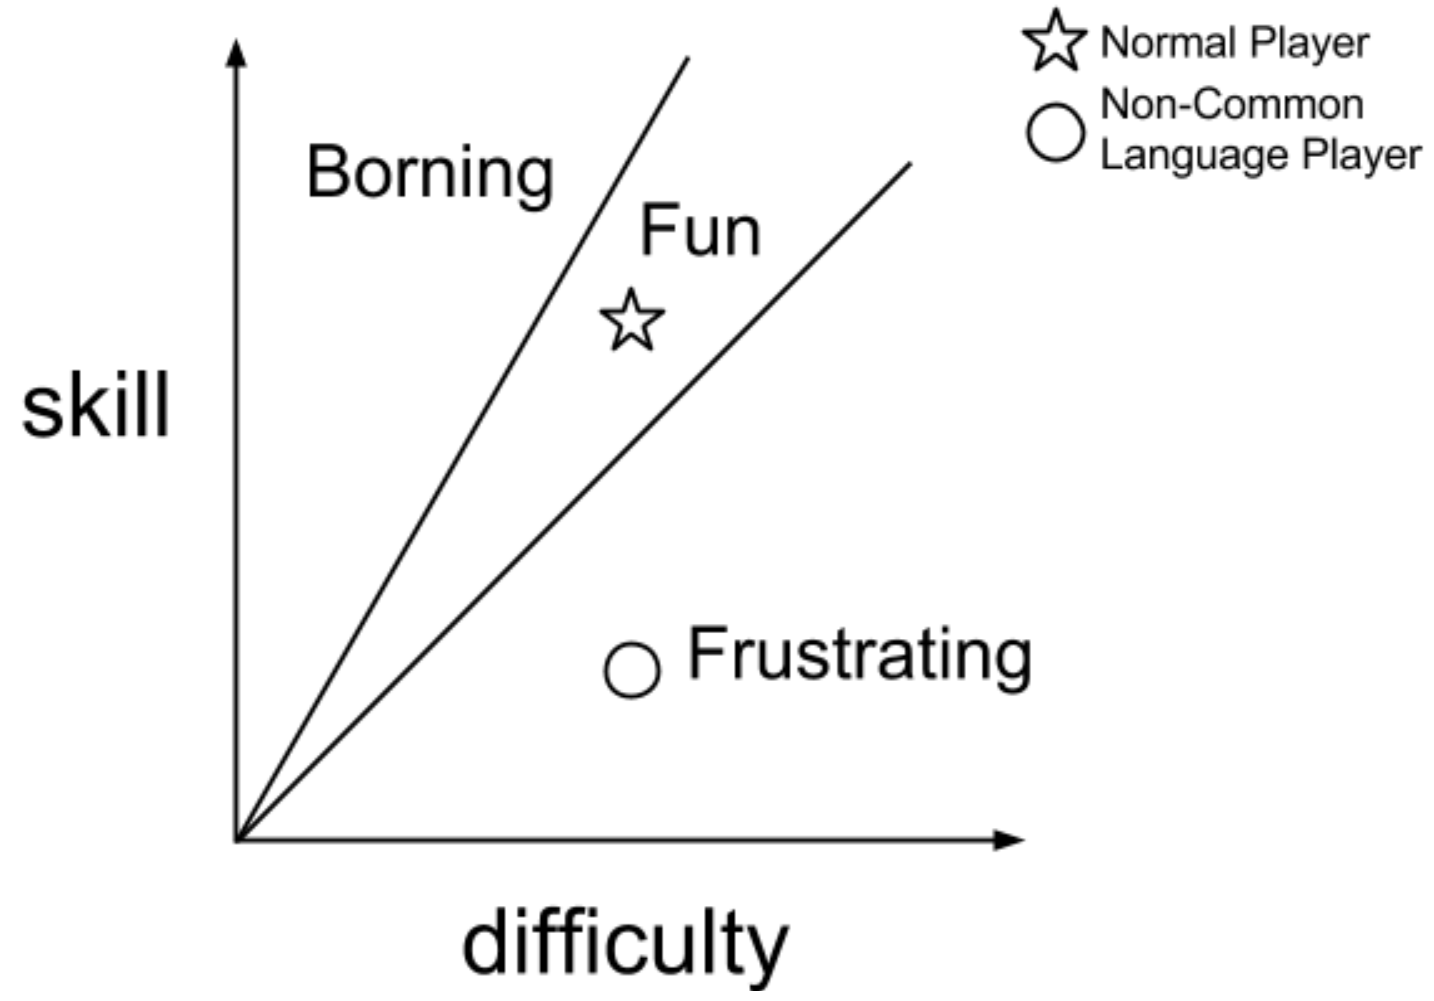
\includegraphics[width=0.9\columnwidth]{Figures/GD_F1.png}
\caption{Language boundary is causing player's skill difference}
\label{fig:GD_F1}
\end{figure}

\subsection{Body Language}

% Human communication involves not only speech, but also a wide variety of gestures and body motions. Body language is the most effective means of communicating un-spoken emotions, a non-verbal way to impart your thoughts without verbalizing it. According to The 7\% Rule [1], communication is only 7 percent verbal and 93 percent non-verbal. The non-verbal component was made up of body language(55 percent) and tone of voice (38 percent).

Consist of human communication, there are not only speech but also inclusive of various gestures and body motions. Body language, a non-verbal way to transmit your thoughts without verbalizing. Accouring to The 7\% Rule\cite{GD2}, the influence for communication for verbal is only 7\% but is 93\% for non-verbal expression. And the non-varbal expression is made up of body language (55\%) and tones of voice (38\%).

% Charades[2] is a word guessing game.In the form most played today, it is an acting game in which one player acts out a word or phrase, often by miming similar sounding words, and the other players guess the word or phrase. The idea is to use physical rather than verbal language to convey the meaning to another party.

Charades\cite{GD3} is a word guessing game. Charades is an acting game in which one player acts as a word or a phrase, and sometime imitates a similar pronounced words, while the other players guess for the answer. The main idea is to use body to make physical expression rather than using verbal language. 

% Inspired by The 7\% Rule and Charades, We suggest to use body language as a communication manner in cooperative game to normalize player’s communication skill, so that no matter players are playing with different language speaker or not, their communication skill is near enough for game developer to design a proper difficulty to please players.

Inspired by The 7\% Rule and the Charades, we suggested to use body language as a communication manner in cooperative game to normalize player's communication skill. With this idea, whether players are playing with different language speakers or not, their communication skill is near enough for game developer to design a proper difficulty to entertain players.


\subsection{Prototype - Mute Robot}

% To explore our idea that using body language communication in cooperative game , we have designed Mute Robot, a game in which 2 players must cooperate to solve a series of puzzle challenges by communicating through body language only.

The main idea we want to explore is the influence of using body language in cooperative game. In order to find out the answer, we had designed Mute Robot, a game in which 2 players must cooperate to solve a series of puzzle challenges by communicating through body language only.

To encourage players to use body language, we have designed an asymmetric puzzle system, with only one player receiving puzzle hints. The player will use body language to guide the other player to solve the puzzle. Taking one of our game stage as an example (see Figure~\ref{fig:GD_F2}), there is a locked door on the right side which obstructs both players’ route to the next stage. The top player can’t see the puzzle-solving hints but can turn the wheel to the match the puzzle answer, which consequently opens the locked door. The only way to pass the stage is for the bottom player to convey the puzzle-solving messages to the other player with body language.

\begin{figure}[!h]
\centering
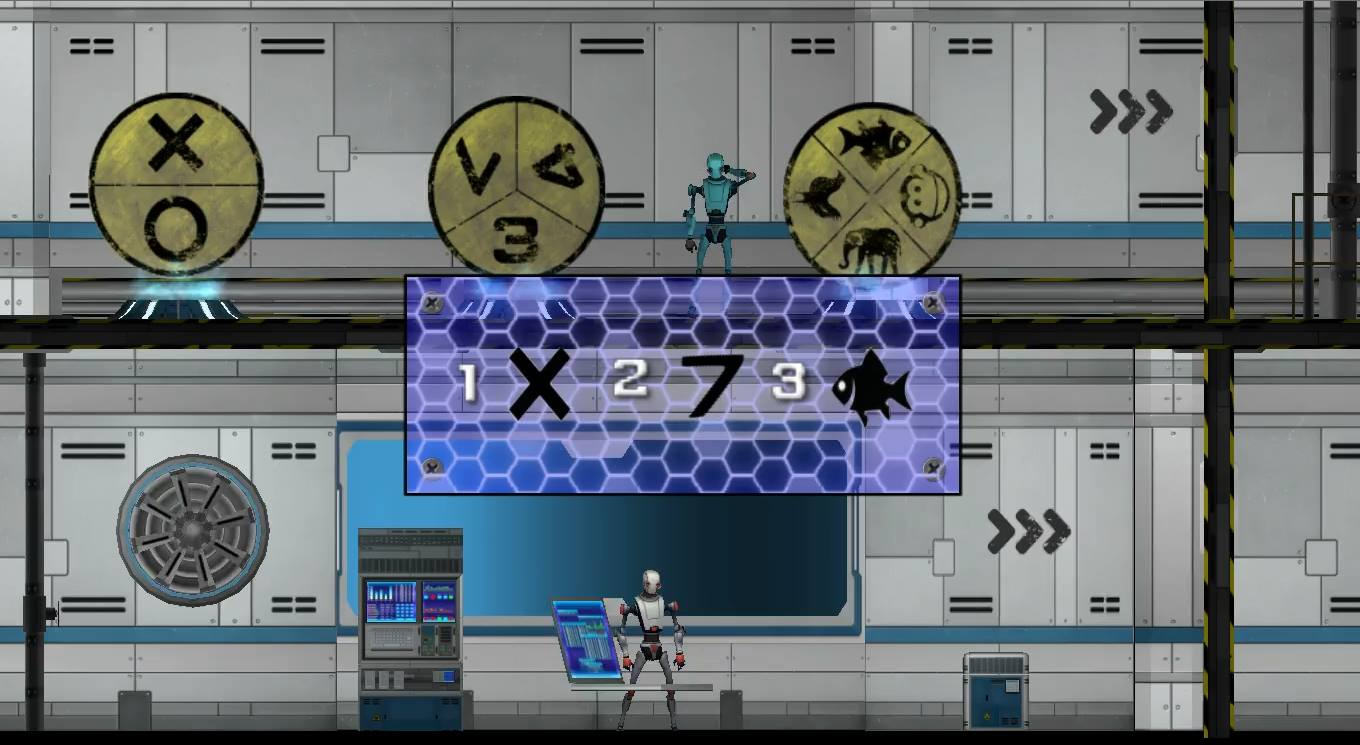
\includegraphics[width=0.9\columnwidth]{Figures/GD_F2.jpg}
\caption{The asymmetric puzzle game design in one of Mute Robot’s stages.}
\label{fig:GD_F2}
\end{figure}


\subsection{Level Design}

% To test the limitation of body language in cooperative game, we designed three puzzles with incremental difficulty. Every message for player to transmit is getting more and more complex.

In order to test the limitation of using body language in cooperative game, we designed three puzzles with incremental difficulty, which means that the message player needed to transmit will have higher complexity than previous one. Next we introduce each game level respectively.

% In the first level, we are testing sequence message to transmit which is a classic cooperative game puzzle. One player has to express the secret sequence to another player, so that he can press the apparatus buttons in correct sequence, then open the door and route to next puzzle.

In the first level, we test sequence messages whether to be transmitted or not. This is a classic puzzle in cooperative game. One player has to express the secret sequence to another player so that another player can press the apparatus buttons in correct order. If the order is correct, the door will open and both players can proceed to the next level.

% In the second level, there are three apparatus wheel to turn to the correct pattern. The symbols on the first wheel are two state of boolean value (circle and cross), and the second wheel’s symbols are numbers (3,4,7), the symbols on the last wheel are animals(fish, chicken, monkey and elephant).

In the second level, there are three apparatus wheels which need to be turned to match the correct pattern. Symbols on the first wheel are boolean value (circle and cross). The second wheel's symbols are numbers (3, 4, 7), and the last wheel's symbols are animals (fish, chicken, monkey and elephant).

% In the last level, we want to test more complex concept like emotion, so we randomly give an emotion word for player to transmit (angry, happy or tired) ,and the player on the other side needs to guess the emotion and spell it correctly.

In the last level, we want to test the concept with higher complexity, such as emtion. So we randomly provide an emotion word (angry, happy or tired) for one player and he needs to transmit to another player. The level can be passed only if another player guess the emotion and spell it correctly.

\subsection{System Implementation}

% Mute Robot is a cooperative puzzle platformer game built using Unity3D[4] engine. The game involves two players at two distinct locations connected over the Internet. The players cannot talk to each other directly and the only way to communicate is using their body language. we use Kinect to capture player’s body language and apply to their avatar. To avoid arm fatigue of mid-air interactions [1] with Kinect, each player uses a Wii[3] controller to complete trivial manipulation (e.g.move left,move right, jump, confirm, cancel). 

Mute Robot is a cooperative puzzle platformer game built using Unity3D\cite{GD4} engine. The game involves two players at two distinct locations connected over the Internet. The players cannot talk to each other directly and the only way to communicate is using their body language. We use Kinect to capture player's body language and apply to their avatar. In order to avoid arm fatigue of mid-air interactions\cite{GD6} with Kinect, each player uses a Wii\cite{GD5} controller to complete trivial manipulation (e.g. move left, move right, confirm, cancel).




\section{Introduction}

\subsection{Abstract and Keywords}


% \begin{figure}[!h]
% \centering
% 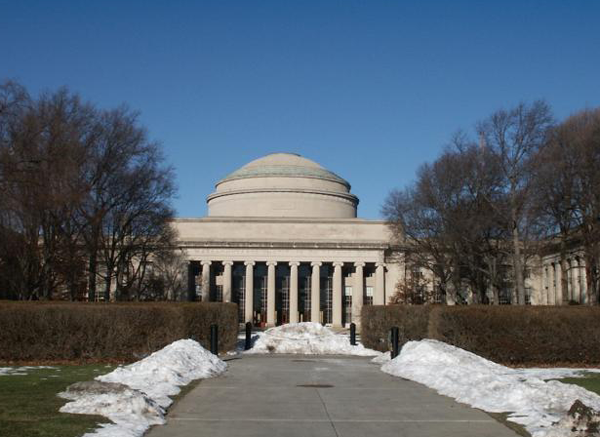
\includegraphics[width=0.9\columnwidth]{Figure1}
% \caption{With Caption Below, be sure to have a good resolution image
%   (see item D within the preparation instructions).}
% \label{fig:figure1}
% \end{figure}

\textit{Proc. Interact 2003}). 
\texttt{References} style

 ``[Robertson, personal communication]''

% \begin{table}
%   \centering
%   \begin{tabular}{|c|c|c|}
%     \hline
%     \tabhead{Objects} &
%     \multicolumn{1}{|p{0.3\columnwidth}|}{\centering\tabhead{Caption --- pre-2002}} &
%     \multicolumn{1}{|p{0.4\columnwidth}|}{\centering\tabhead{Caption --- 2003 and afterwards}} \\
%     \hline
%     Tables & Above & Below \\
%     \hline
%     Figures & Below & Below \\
%     \hline
%   \end{tabular}
%   \caption{Table captions should be placed below the table.}
%   \label{tab:table1}
% \end{table}


\section{Figures/Captions}

(see Figure~\ref{fig:figure1}). 
``Table~\ref{tab:table1}'' or ``Figure~\ref{fig:figure2}''), 

\begin{itemize}
\item Write in a straightforward style.
\end{itemize}

\begin{enumerate}
	\item Add alternative text to all figures
	\item Mark table headings
\end{enumerate}



% Balancing columns in a ref list is a bit of a pain because you
% either use a hack like flushend or balance, or manually insert
% a column break.  http://www.tex.ac.uk/cgi-bin/texfaq2html?label=balance
% multicols doesn't work because we're already in two-column mode,
% and flushend isn't awesome, so I choose balance.  See this
% for more info: http://cs.brown.edu/system/software/latex/doc/balance.pdf
%
% Note that in a perfect world balance wants to be in the first
% column of the last page.
%
% If balance doesn't work for you, you can remove that and
% hard-code a column break into the bbl file right before you
% submit:
%
% http://stackoverflow.com/questions/2149854/how-to-manually-equalize-columns-
% in-an-ieee-paper-if-using-bibtex
%
% Or, just remove \balance and give up on balancing the last page.
%
\balance

\section{References format}
References must be the same font size as other body text.
% REFERENCES FORMAT
% References must be the same font size as other body text.

\bibliographystyle{acm-sigchi}
\bibliography{sample}
\end{document}
